%----------------------------------------------------------------------------------------
%	PACKAGES
%----------------------------------------------------------------------------------------

\documentclass[paper=a4, fontsize=11pt]{scrartcl} % A4 paper and 11pt font size
\usepackage{fourier} % Use the Adobe Utopia font for the document - comment this line to return to the LaTeX default
% \usepackage[english]{babel} % English language/hyphenation
\usepackage[ngerman]{babel}
\usepackage{amsmath,amsfonts,amsthm,amssymb} % Math packages
\usepackage{graphicx}
\usepackage[utf8]{inputenc}
\usepackage{wasysym}
\usepackage{enumitem}
\usepackage{stmaryrd}
\usepackage{wrapfig}
\usepackage{siunitx}
\usepackage{tabularx}
\usepackage{listings}
\usepackage{float}
\usepackage{caption}
\usepackage{subcaption}
\usepackage{pdfpages}
\usepackage{lscape}
\usepackage{geometry}
\usepackage{sectsty} % Allows customizing section commands
\usepackage{fancyhdr} % Custom headers and footers

%----------------------------------------------------------------------------------------
%	DOCUMENT CONFIGURATIONS
%----------------------------------------------------------------------------------------

\geometry{a4paper, portrait, margin=1.0in}
\selectlanguage{ngerman}
% \allsectionsfont{\centering \normalfont\scshape} % Make all sections centered, the default font and small caps

\pagestyle{fancyplain} % Makes all pages in the document conform to the custom headers and footers
\fancyhead[L]{Verena Dittmer, Mario Graf} % Page header
\fancyhead[R]{SS 2015 Verteilte Systeme} % Page header
\fancyfoot[L]{} % Empty left footer
\fancyfoot[C]{} % Empty center footer
\fancyfoot[R]{Seite~\thepage} % Page numbering for right footer
\renewcommand{\headrulewidth}{0pt} % Hide header underlines
\renewcommand{\footrulewidth}{0pt} % Hide footer underlines
\setlength{\headheight}{13.6pt} % Customize the height of the header
% \fancyheadoffset{0cm} 

\setlength{\parskip}{\baselineskip}%
\setlength{\parindent}{0pt}%

\numberwithin{equation}{section} % Number equations within sections (i.e. 1.1, 1.2, 2.1, 2.2 instead of 1, 2, 3, 4)
\numberwithin{figure}{section} % Number figures within sections (i.e. 1.1, 1.2, 2.1, 2.2 instead of 1, 2, 3, 4)
\numberwithin{table}{section} % Number tables within sections (i.e. 1.1, 1.2, 2.1, 2.2 instead of 1, 2, 3, 4)

% \setlength\parindent{0pt} % Removes all indentation from paragraphs - comment this line for an assignment with lots of text
\setlength{\parskip}{1em} % set vertical spacing of parahraphs

\lstdefinestyle{base}{
  language=C,
  emptylines=1,
  breaklines=true,
  basicstyle=\ttfamily\color{black},
  commentstyle=\ttfamily\color{black},
  keywordstyle=\ttfamily\color{black},
  numberstyle=\ttfamily\color{black},
  stringstyle=\ttfamily\color{black},
  showstringspaces=false
}

%----------------------------------------------------------------------------------------
%	TITLE SECTION
%----------------------------------------------------------------------------------------

\newcommand{\horrule}[1]{\rule{\linewidth}{#1}} % Create horizontal rule command with 1 argument of height

\title{	
\normalfont \normalsize 
% \textsc{Alpe-Adria Universität Klagenfurt} \\ [25pt] % Your university, school and/or department name(s)
% \horrule{0.5pt} \\[0.4cm] % Thin top horizontal rule
\huge Bildersuche mit Hadoop und MapReduce\ % The assignment title
\horrule{0.2pt} % Thick bottom horizontal rule
}

\author{Verena Dittmer, Mario Graf} % Your name

\date{\normalsize\today} % Today's date or a custom date

\begin{document}
\maketitle % Print the title
\lstset{style=base}

\section{Umsetzung}

Wir haben unsere Implementierung in zwei Module aufgeteilt: \lstinline$hd-image-search-core$ und \lstinline$hd-image-search-gui$. Als Feature wurde Lire's CEDD Feature verwendet. Um die Distanzen zu berechnen wurde die Euklidische Distanz eingesetzt.

Die Vollständige Implementierung ist unter GitHub erreichbar:
\begin{lstlisting}
https://github.com/hawk23/hd-image-search
\end{lstlisting}

\subsection{hd-image-search-core}
Dieses Modul beinhaltet die MapReduce Task um Features zu extrahieren und für die Bildsuche an sich. Das zugehörige jar File \lstinline$hd-core.jar$ bedfindet sich im Ordner \lstinline$jars$.

\subsubsection{Verwendung}
Um die MapReduce tasks in einem Hadoop Cluster ausführen zu können muss das entsprechende jar file zuerst bekannt gegeben werden:
\begin{lstlisting}
$ export HADOOP_CLASSPATH=/home/hduser/jars/hd-core.jar
\end{lstlisting}

Features können mit folgendem Befehl extrahiert werden. Der erste Parameter ist der Ordner im Hadoop Cluster der die Bilder beinhaltet, der zweite Parameter ist der Ordner in dem dann die Indexdatei erstellt werden soll.
\begin{lstlisting}
$ hadoop hdimagesearch.core.FeatureExtract /images/png2 /index
\end{lstlisting}

Um ein Bildsuche zu starten können folgende Befehle ausgeführt werden. Als erster Parameter muss man den Ordner angeben in dem sich der Index befindet, dann den Ordner in dem das Suchergebnis gespeichert werden soll. Mit \lstinline$-n$ kann man die Anzahl der gewünschten Suchergenisse angeben. Als Suchbild kann man entweder ein bereits im Hadoop Cluster gespeichertes Bild angeben (\lstinline$-h "/images/png2/1/1_i110.png"$) oder einen Featurestring, wenn man bereits die Features eines Bildes extrahiert hat (\lstinline$-f "1.0;3.0:1.0;0.0;....."$).

\begin{lstlisting}
$ hadoop hdimagesearch.core.ImageSearch /index /searchResult -n 10 -h "/images/png2/1/1_i110.png"
$ hadoop hdimagesearch.core.ImageSearch /index /searchResult -n 10 -f "1.0;3.0:1.0;0.0;..."
\end{lstlisting}

Anschließend kann man sich das Ergebnis der Suche anzeigen lassen:
\begin{lstlisting}
$ hadoop fs -cat /searchResult/part-r-00000
$ 
$ 0.0        hdfs://localhost:54310/images/png2/1/1_i110.png
$ 1.41421356 hdfs://localhost:54310/images/png2/1/1_i120.png
$ 1.73205080 hdfs://localhost:54310/images/png2/1/1_i130.png
$ 2.0        hdfs://localhost:54310/images/png2/1/1_i140.png
$ 2.23606797 hdfs://localhost:54310/images/png2/1/1_i150.png
$ 3.0        hdfs://localhost:54310/images/png2/1/1_i160.png
$ 3.60555127 hdfs://localhost:54310/images/png2/1/1_i170.png
$ 3.87298334 hdfs://localhost:54310/images/png2/1/1_i180.png
$ 4.69041575 hdfs://localhost:54310/images/png2/1/1_i230.png
$ 4.69041575 hdfs://localhost:54310/images/png2/1/1_i190.png
\end{lstlisting}

\subsection{hd-image-search-gui}
Diese Modul beinhaltet die grafische Benutzeroberfläche um Features zu extrahieren und um eine Bildsuche durchzuführen. Das Modul baut auf \lstinline$hd-image-search-core$ auf und nutzt die dort definierten MapReduce Tasks. Das jar file, mit dem sich die Benutzeroberfläche starten lässt, findet man unter \lstinline$jars/hd-gui.jar$.

Gestartet werden kann die GUI einfach mit:
\begin{lstlisting}
$ java -jar hd-gui.jar 
\end{lstlisting}

Zuerst muss man auswählen auf welchem Cluster man die Operationen ausführen mächte. Im oberen Bereich der Benutzeroberfläche findet man dazu eine Auswahlbox um die gewünschte Clusterkonfiguration auszuwählen. Über den Button \emph{Add Config ...} kann man schnell eine neue Konfiguration anlegen.

Um Features extrahieren zu könne muss man unter dem Tab \emph{Feature Extract} auf den Button \emph{Extract Features} klicken. Im Log Fenster im unteren Bereich der Oberfläche werden Logeinträge zu Erfolgs- und Fehlerfällen ausgegeben (Abbildung \ref{fig:s1}).

Für die Bildersuche muss zuerst unter dem Tab \emph{Search} mittels \emph{Select Image ...} ein Bild aus dem lokalen Dateisystem ausgewählt werden. Das Bild wird als Vorschau rechts neben den Einstellungen angezeigt. Weiters kann man auch die Anzahl der gewünschten Ergebnisse angeben. Mit einem Klick auf \emph{Start Search} kann die Suche gestartet werden und die Ergebnisse werden angezeigt (Abbildung \ref{fig:s2}).

\begin{figure}[H]
\begin{center}
	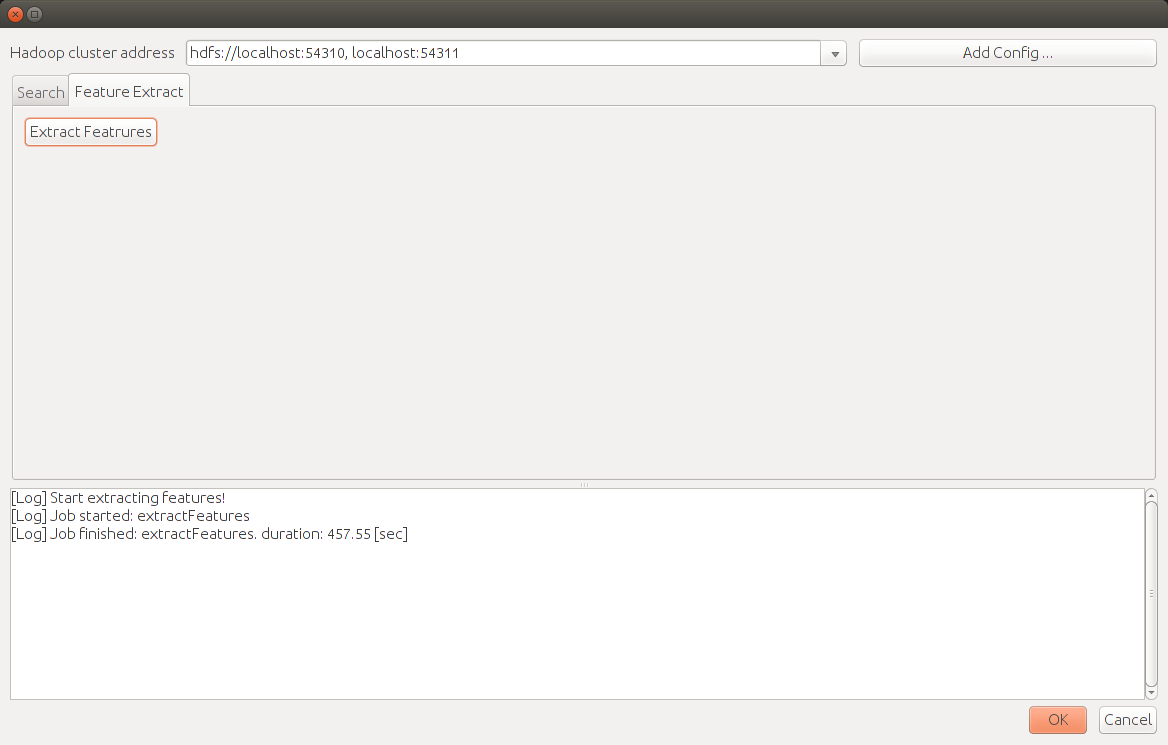
\includegraphics[width=\textwidth]{images/screen1}
	\caption{Eingabemaske um Features zu extrahieren.}
	\label{fig:s1}
\end{center}
\end{figure}

\begin{figure}[H]
\begin{center}
	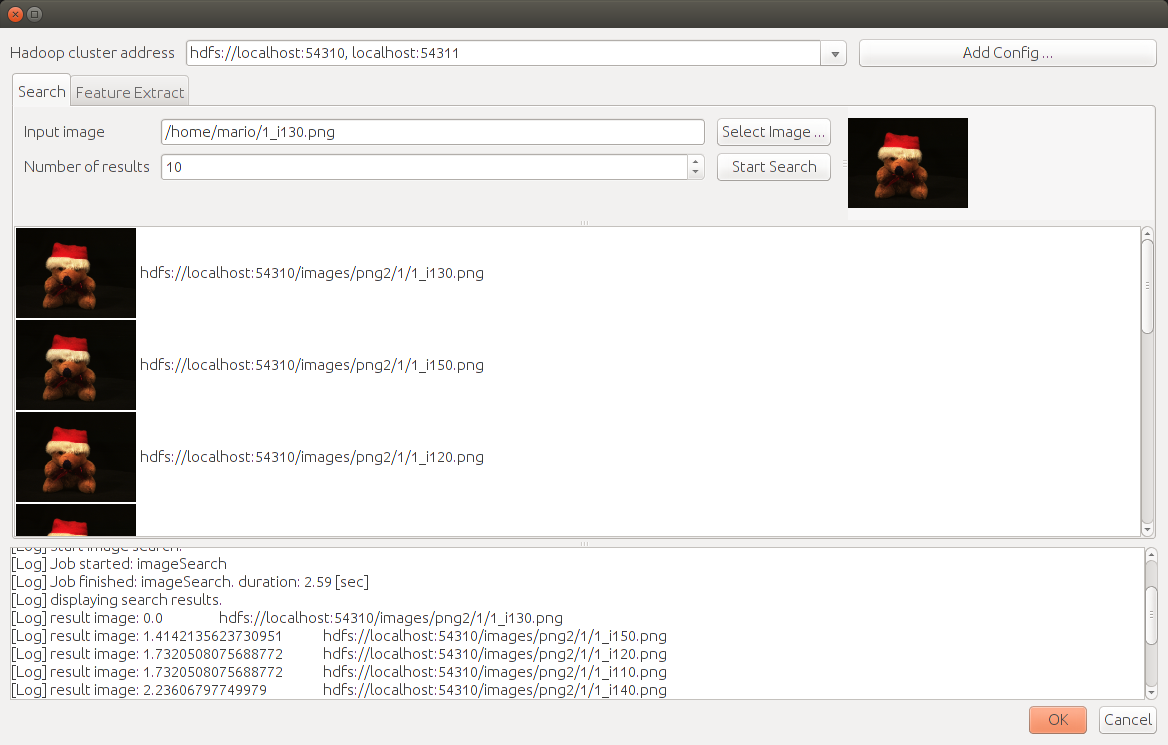
\includegraphics[width=\textwidth]{images/screen2}
	\caption{Eingabemaske um eine Bildersuche zu starten.}
	\label{fig:s2}
\end{center}
\end{figure}

\section{Erledigte Aufgaben}
Von den zu erledigenden Aufgaben haben wir alle Plichtaufgaben (1. - 4.) erfüllt. Von den Zusatzaufgaben haben wir umgesetzt:

\begin{itemize}
\item Modify your code from task 4 so that the returned result contains 10 of the most similar images and their distance index.
\item Implement a GUI where the user can search for similar image by loading an image
from its local system. Once the search completes the user should be able to see the
10 most similar images.
\item Test your code in a fully distributed environment using one of the following
techniques.
	\begin{itemize}
	\item Use our provided servers to test your code in a fully distributed environment.
	\item Set up a fully distributed cluster and test your implementation there.
	\end{itemize}
\item Increase the number of nodes in the cluster and check the performance of your code
with 1, 2, 3, 4 or more different nodes.
\end{itemize}

\end{document}

